% Chapter Template

\chapter{Using STUFF to do THINGS} % Main chapter title

\label{Chapter5} % Change X to a consecutive number; for referencing this chapter elsewhere, use \ref{ChapterX}

%-----------------------------------------------------------
\section{Main Section 1}
%-----------------------------------------------------------

Lorem ipsum dolor sit amet, consectetur adipiscing elit. Aliquam ultricies lacinia euismod. Nam tempus risus in dolor rhoncus in interdum enim tincidunt. Donec vel nunc neque. In condimentum ullamcorper quam non consequat. Fusce sagittis tempor feugiat. Fusce magna erat, molestie eu convallis ut, tempus sed arcu. Quisque molestie, ante a tincidunt ullamcorper, sapien enim dignissim lacus, in semper nibh erat lobortis purus. Integer dapibus ligula ac risus convallis pellentesque.

%---------------------------------------
\subsection{Subsection 1}
%---------------------------------------

Nunc posuere quam at lectus tristique eu ultrices augue venenatis. Vestibulum ante ipsum primis in faucibus orci luctus et ultrices posuere cubilia Curae; Aliquam erat volutpat. Vivamus sodales tortor eget quam adipiscing in vulputate ante ullamcorper. Sed eros ante, lacinia et sollicitudin et, aliquam sit amet augue. In hac habitasse platea dictumst.




I am able to construct a model of lower mantle heat flux, including the effect of LLSVP properties. Using LEMA, I specify a CMB base condition, and a TBL condition at some height above it. In all models I consider, the CMB will be isothermal. The TBL will have a variable mean temperature, and regions of higher and lower temperature. The lower mantle has an average Fe\%, but the LLSVPs are enriched compared the depleted surrounding bulk lower mantle. By varying the temperature and composition at the CMB, conductivity can be altered using the model from PREVIOUS-REF. The difference in temperature between CMB and TBL, and the undulations on the latter, control the lower mantle temperature gradient. 

Heat flux can be calculated using conductivity and temperature gradient via FOURIER'S LAW. While the magnitude of the heat flux will change with parameters, perhaps more interesting is the lateral variation of this parameter. This will show how the lower mantle heat flux is sensitive to the conditions therein, and what condition or combination of conditions is most significant. The results from these calculations can then be compared to observables, dismissing scenarios which are unfeasible or unstable. There are many variables in the lower mantle, and observables to compare to. The variable conductivities from this work will play an important role in constraining CMB heat flux.

I can use spherical harmonics to generate structures that resemble LLSVPs. The centre of LLSVPs are approximately(/loosely?) located on the equator, antipodal at $0\degsym$ and $180\degsym$ longitude (the African and Pacific LLSVPs respectively). A first order approxiamtion for this geometry is the spherical harmonic $Y^{2}_{2}$, four quadrants of varying polarity around the polar axis. This looks good, but the projection is misleading in that it actually extends to the poles. It can be improved by stacking $Y^{0}_{2}$ on top of it, enhancing regions on the equator and reducing everything towards the poles. The results is two circular patterns, each located at opposite sides of the equator.

%$Y^{m}_{l}$

\begin{figure}[h]
  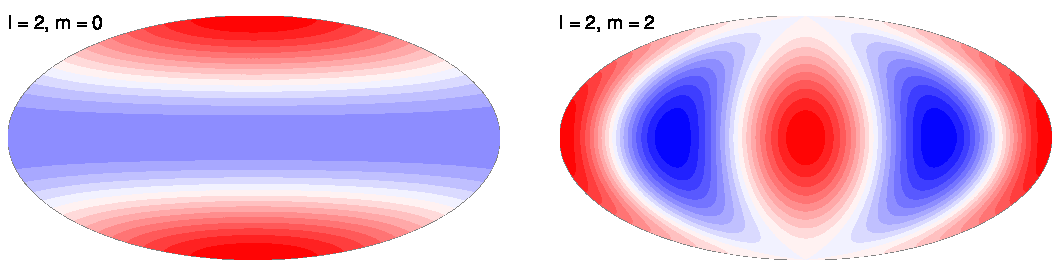
\includegraphics[width=\linewidth]{Figures/sph_harm.png}
  \caption[SPHERICAL HARMONICS]{Source: http://www-udc.ig.utexas.edu/external/becker/teaching-sh.html
  
These two harmonics are added together, amplifying blue regions on the equator, and diminshing everything else.}
  \label{fig:spherical_harmonics_diagram}
\end{figure}

For the $Y^{2}_{2}$ pattern, the areas of positive and negative amplitude regions are equal. For the  $Y^{0}_{2}$-combined model, the distribution of polarities is not even. By the way something like temperature is set up in the model, having a mean value with a ``$\pm$'' range leads to hotter hots, and warmer colds. There is more of the cold, surrounding mantle compared to LLSVP-designated regions, the LLSVPs have to be hotter than the surrounding mantle is colder.

Conductivity cannot be probed from the surface, but seismic velocities can be inferred from tomography. The same processes that affect conductivity generally affect shear wave velocity in the same fashion, be it increase or decrease. I can use $V_{\mathrm{S}}$ observations as an analogue to make inferences about the lower mantle.

When conductivity is kept constant across the whole CMB, variations in heat flux are determined solely by the lower mantle temperature profile. The reverse is also true, with constant temperature gradient above the CMB, conductivity controls lateral heat flow variations. This is a vast oversimplification, just talking about possible endmembers, in reality there will be both temperature and compositional factors affecting heat flux. Conductivity itself is temperature-dependent, further tying the two variables together.

When modelling LLSVPs, we are assuming they are thermochemical piles, that they are hotter and denser (e.g. high Fe\%) than the surrounding lower mantle. Increasing temperature reduces conductivity, as does increasing impurity inclusion. By modelling LLSVPs as purely thermal piles (i.e. increasing their temperature), we see a reduction in heat flux. This flux is further reduced when Fe content is increased, as conductivity decreases with impurity content. By altering temperature and composition in tandem, I will be able to suggest sets of lower mantle conditions which reproduce observations.

While this model is of dubious use in constraining the exact nature of CMB heat flux, inferences can be made on the relative variations laterally. How much heat is impeded passing through a LLSVP? How extreme do temperature and compositional variations need to be to significantly affect the distribution of heat flow? An important parameter will be that of the lateral variation in heat flux
%
\begin{equation}
\label{eq.q_star}
q* = \frac{q_{\mathrm{max}}-q_{\mathrm{min}}}{q_{\mathrm{mean}}}\ ,
\end{equation}
%
where max and min refer to the calculated extremes, and mean the average over the whole CMB. The larger the value of $q*$, the smaller the heat flux through the LLSVPs. While the magnitudes of heat flux may not be accurate, using $q*$ will let me make comments on thermal conductivity's role in the Earth heat engine for a wide range of possible lower mantle conditions.




%VARIABLES TO PLAY WITH

%Temp_cmb
%Temp_tbl
%Temp_diff
%Temp_hot
%Temp_cold

%Height_tbl
%Height_llsvp (peak height, how is shape considered, sph. harm.?)

%Comp_mean
%Comp_lm
%Comp_llsvp
